%%%%%%%%%%%%%%%%%%%%%%%%%%%%%%%%%%%%%%%%%
% Beamer Presentation
% LaTeX Template
% Version 1.0 (10/11/12)
%
% This template has been downloaded from:
% http://www.LaTeXTemplates.com
%
% License:
% CC BY-NC-SA 3.0 (http://creativecommons.org/licenses/by-nc-sa/3.0/)
%
%%%%%%%%%%%%%%%%%%%%%%%%%%%%%%%%%%%%%%%%%

%----------------------------------------------------------------------------------------
%	PACKAGES AND THEMES
%----------------------------------------------------------------------------------------

\documentclass{beamer}

\mode<presentation> {

% The Beamer class comes with a number of default slide themes
% which change the colors and layouts of slides. Below this is a list
% of all the themes, uncomment each in turn to see what they look like.

%\usetheme{default}
%\usetheme{AnnArbor}
%\usetheme{Antibes}
%\usetheme{Bergen}
%\usetheme{Berkeley}
%\usetheme{Berlin}
%\usetheme{Boadilla}
% \usetheme{CambridgeUS}
%\usetheme{Copenhagen}
%\usetheme{Darmstadt}
%\usetheme{Dresden}
%\usetheme{Frankfurt}
%\usetheme{Goettingen}
%\usetheme{Hannover}
%\usetheme{Ilmenau}
%\usetheme{JuanLesPins}
%\usetheme{Luebeck}
\usetheme{Madrid}
%\usetheme{Malmoe}
%\usetheme{Marburg}
%\usetheme{Montpellier}
% \usetheme{PaloAlto}
%\usetheme{Pittsburgh}
%\usetheme{Rochester}
%\usetheme{Singapore}
%\usetheme{Szeged}
%\usetheme{Warsaw}

% As well as themes, the Beamer class has a number of color themes
% for any slide theme. Uncomment each of these in turn to see how it
% changes the colors of your current slide theme.

%\usecolortheme{albatross}
%\usecolortheme{beaver}
%\usecolortheme{beetle}
%\usecolortheme{crane}
%\usecolortheme{dolphin}
%\usecolortheme{dove}
%\usecolortheme{fly}
%\usecolortheme{lily}
%\usecolortheme{orchid}
\usecolortheme{rose}
%\usecolortheme{seagull}
%\usecolortheme{seahorse}
%\usecolortheme{whale}
%\usecolortheme{wolverine}

%\setbeamertemplate{footline} % To remove the footer line in all slides uncomment this line
%\setbeamertemplate{footline}[page number] % To replace the footer line in all slides with a simple slide count uncomment this line

%\setbeamertemplate{navigation symbols}{} % To remove the navigation symbols from the bottom of all slides uncomment this line
}

\usepackage{graphicx} % Allows including images
\graphicspath{{./fig/}}
\DeclareGraphicsExtensions{.pdf,.jpeg,.png}
\usepackage{booktabs} % Allows the use of \toprule, \midrule and \bottomrule in tables
\usepackage[numberedbib]{apacite}
\usepackage[export]{adjustbox}

%----------------------------------------------------------------------------------------
%	TITLE PAGE
%----------------------------------------------------------------------------------------

\title[Online POMDP Planning]
{Online POMDP Planning\\
\vspace{5mm}
(Robotics Workshop at Lab 1231, CS UI)
}

\author{Vektor Dewanto} % Your name
\institute[None] % Your institution as it will appear on the bottom of every slide, may be shorthand to save space
{
Affiliation: None\\ % Your institution for the title page
\medskip
\textit{vektor.dewanto@gmail.com } % Your email address
}
\date{\today} % Date, can be changed to a custom date

\begin{document}

\begin{frame}
\titlepage % Print the title page as the first slide
\end{frame}

\begin{frame}
\frametitle{Outline} % Table of contents slide, comment this block out to remove it
\tableofcontents % Throughout your presentation, if you choose to use \section{} and \subsection{} commands, these will automatically be printed on this slide as an overview of your presentation
\end{frame}

%----------------------------------------------------------------------------------------
%	PRESENTATION SLIDES
%----------------------------------------------------------------------------------------
%%%%%%%%%%%%%%%%%%%%%%%%%%%%%%%%%%%%%%%%%%%%%%%%%%%%%%%%%%%%%%%%%%%%%%%%%%%%%%%
\section{Introduction}
\frame{\tableofcontents[currentsection, hideothersubsections]}

\begin{frame}
\frametitle{Introduction}

\begin{figure}
    \centering
    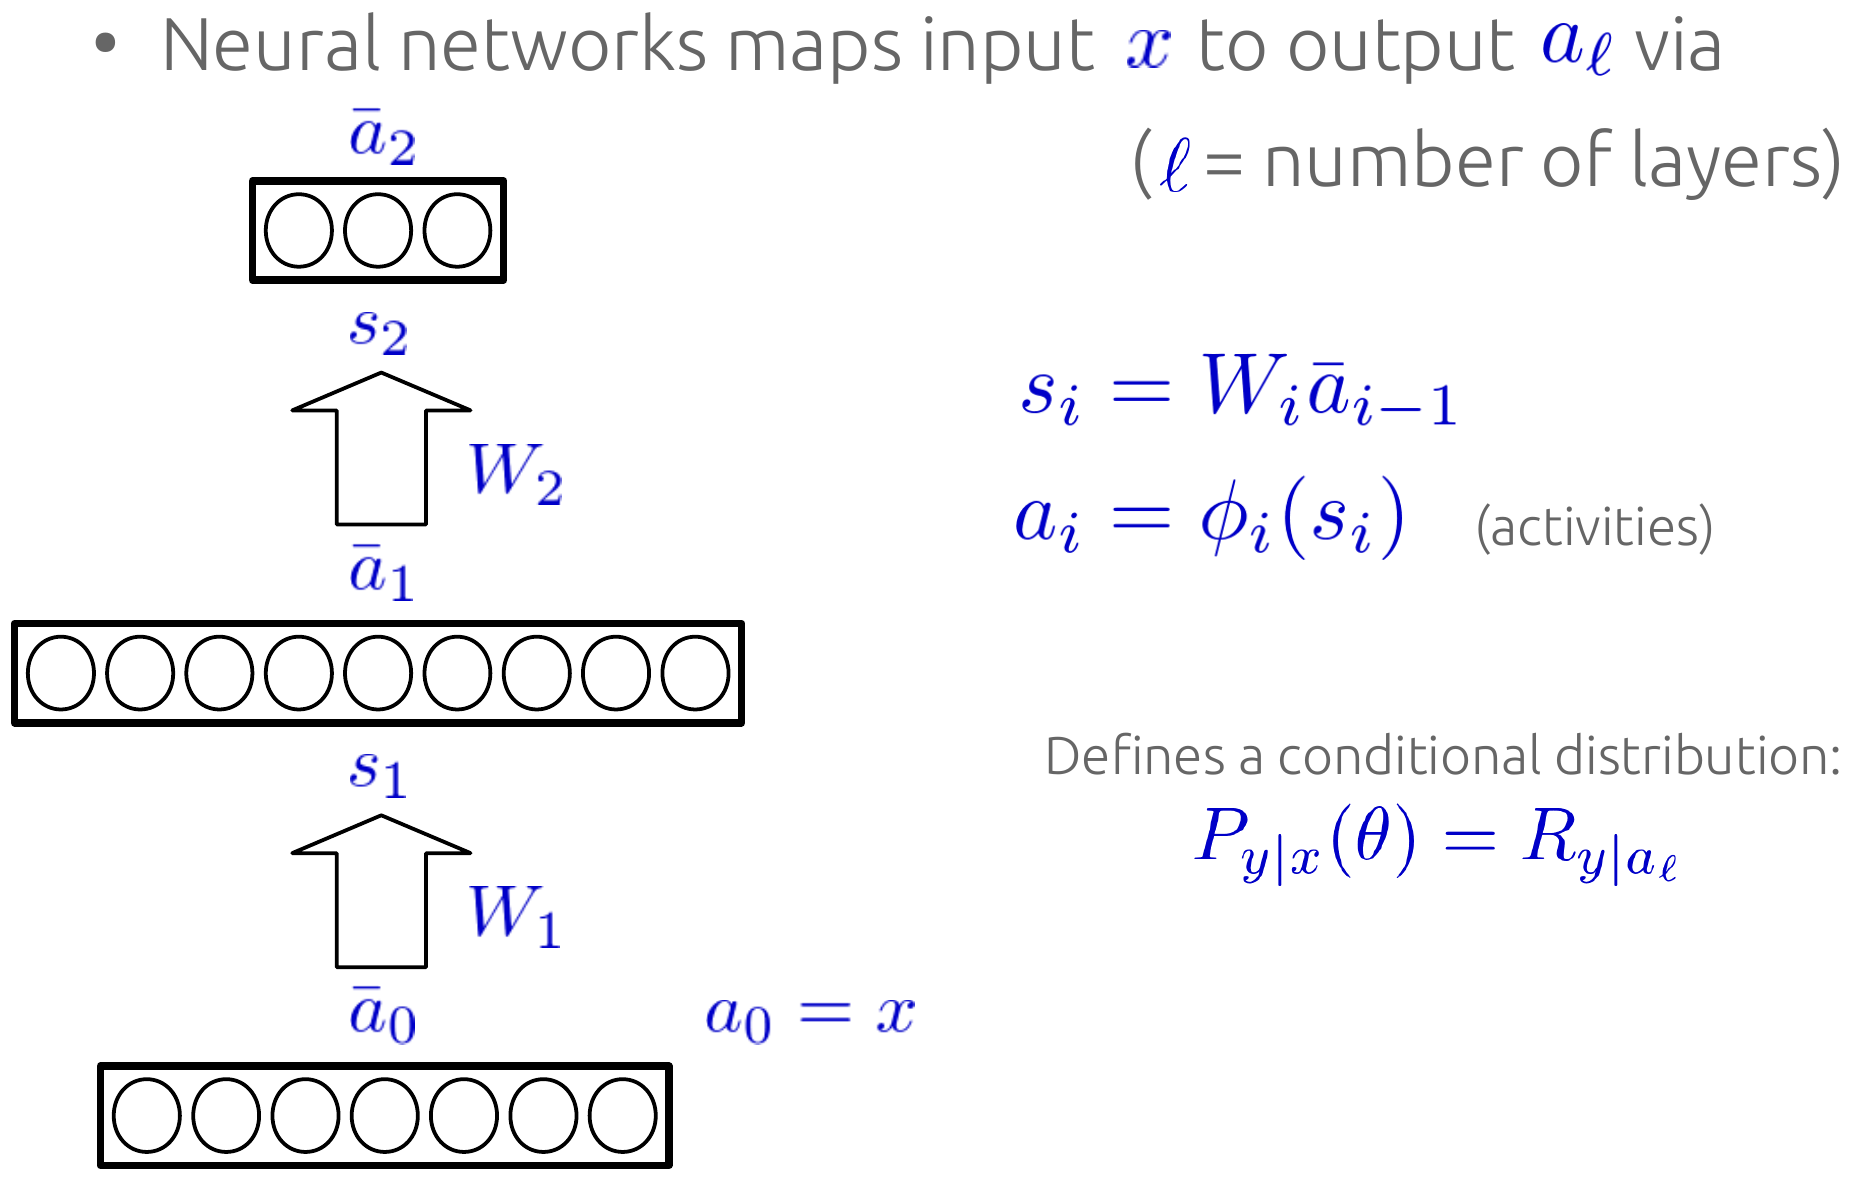
\includegraphics[scale=0.2]{net}
\end{figure}

\begin{itemize}
    \item $\bar{a}_i$ is $a_i$ appended by a homogeneous coordinate with value 1, ie
            to capture bias parameters explicitly
\end{itemize}
\end{frame}

\begin{frame}
\frametitle{Introduction}

\begin{figure}
    \centering
    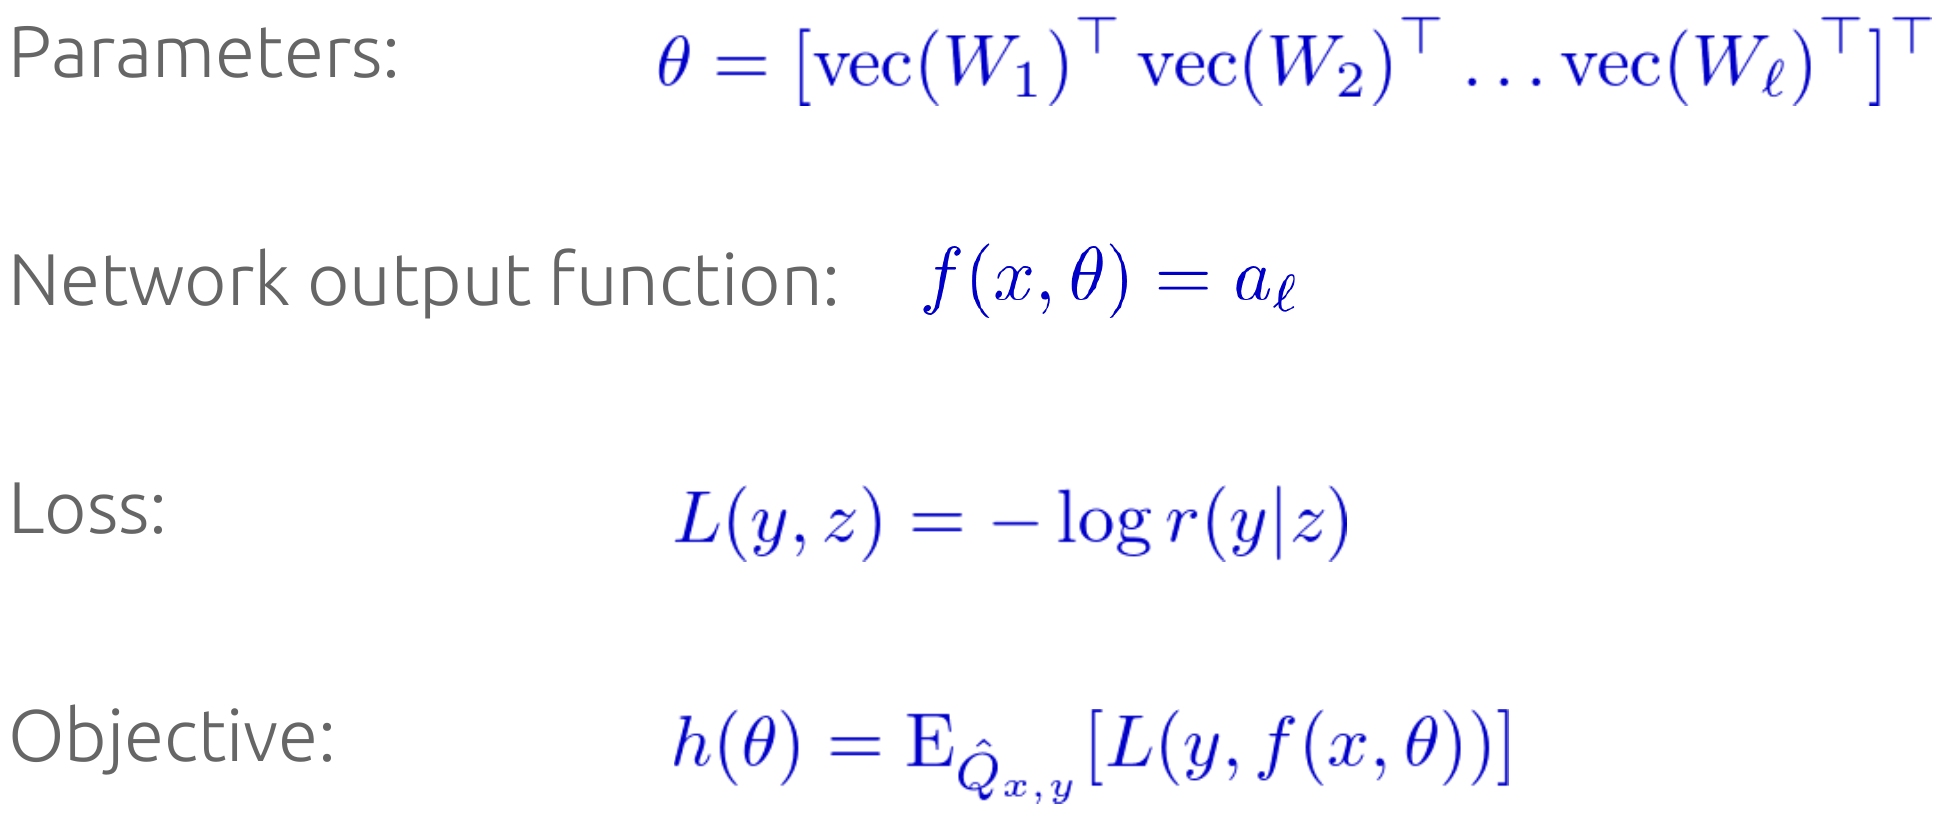
\includegraphics[scale=0.2]{net_param}
\end{figure}

\begin{itemize}
    \item $vec$ vectorizes matrices by stacking their columns together
    \item $\hat{Q}_{x, y}$ is a training distribution
    \item $p(y|x, \theta) = r(y|f(x, \theta))$ is the density function of $P_{y|x}(\theta) = R_{y|f(x,\theta)}$
    \item minimizing $h(\theta)$ can be seen as maximum likelihood learning of~$P_{y|x}(\theta)$.
\end{itemize}

\end{frame}

\begin{frame}
\frametitle{Introduction}
Newton-type update: $\theta_{k+1} = \theta_k - \alpha_k (\nabla^2 h)^{-1} \nabla h$
% \begin{itemize}
%     \item Newton-type update: $\theta_{t+1} = \theta_t - \alpha (\nabla^2 h)^{-1} \nabla h$
% \end{itemize}
\begin{figure}
    \raggedright
    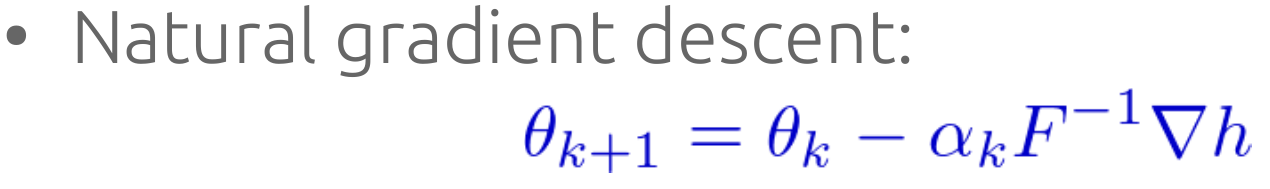
\includegraphics[scale=0.25]{natgrad}
\end{figure}

\begin{figure}
    \raggedright
    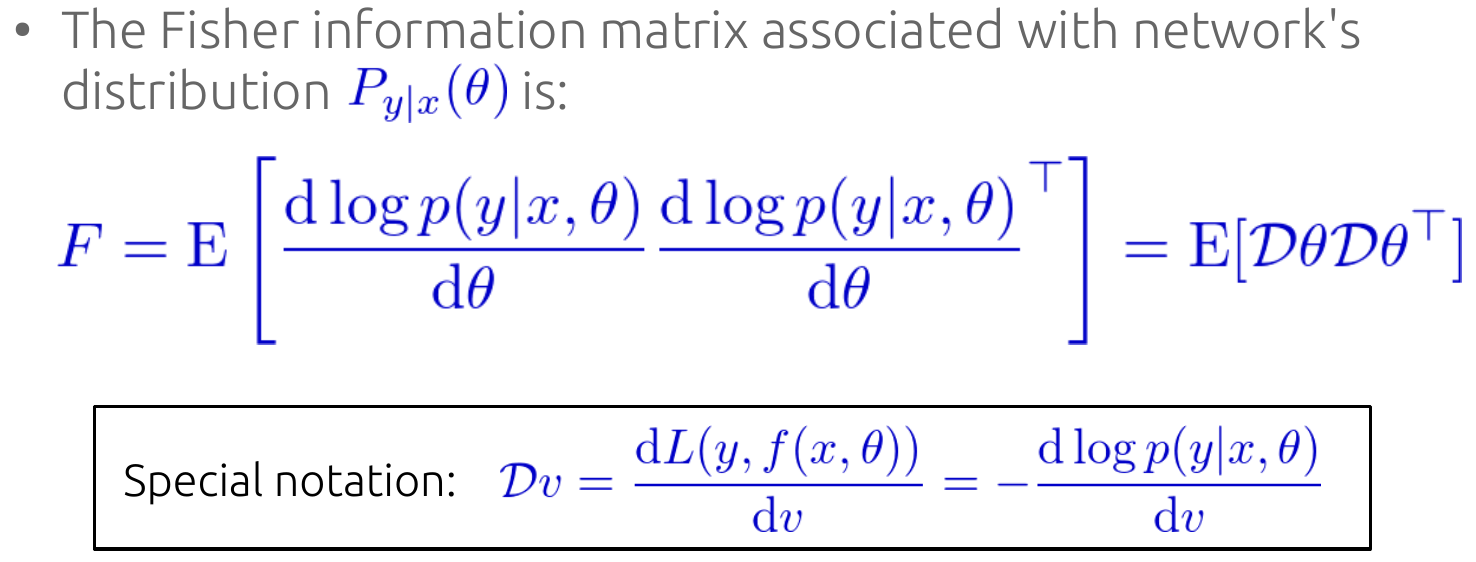
\includegraphics[scale=0.25]{fisher}
\end{figure}

\end{frame}

\section{Monte Carlo Tree Search (MCTS)}
\frame{\tableofcontents[currentsection, hideothersubsections]}

\begin{frame}
\frametitle{Monte Carlo Tree Search (MCTS)}
Based on 2 fundamental concepts:
\begin{itemize}
\item {\small the true value of an action may be approximated using random simulation}
\item these approximated values may be used efficiently to adjust the policy
\end{itemize}

\begin{figure}
    \centering
    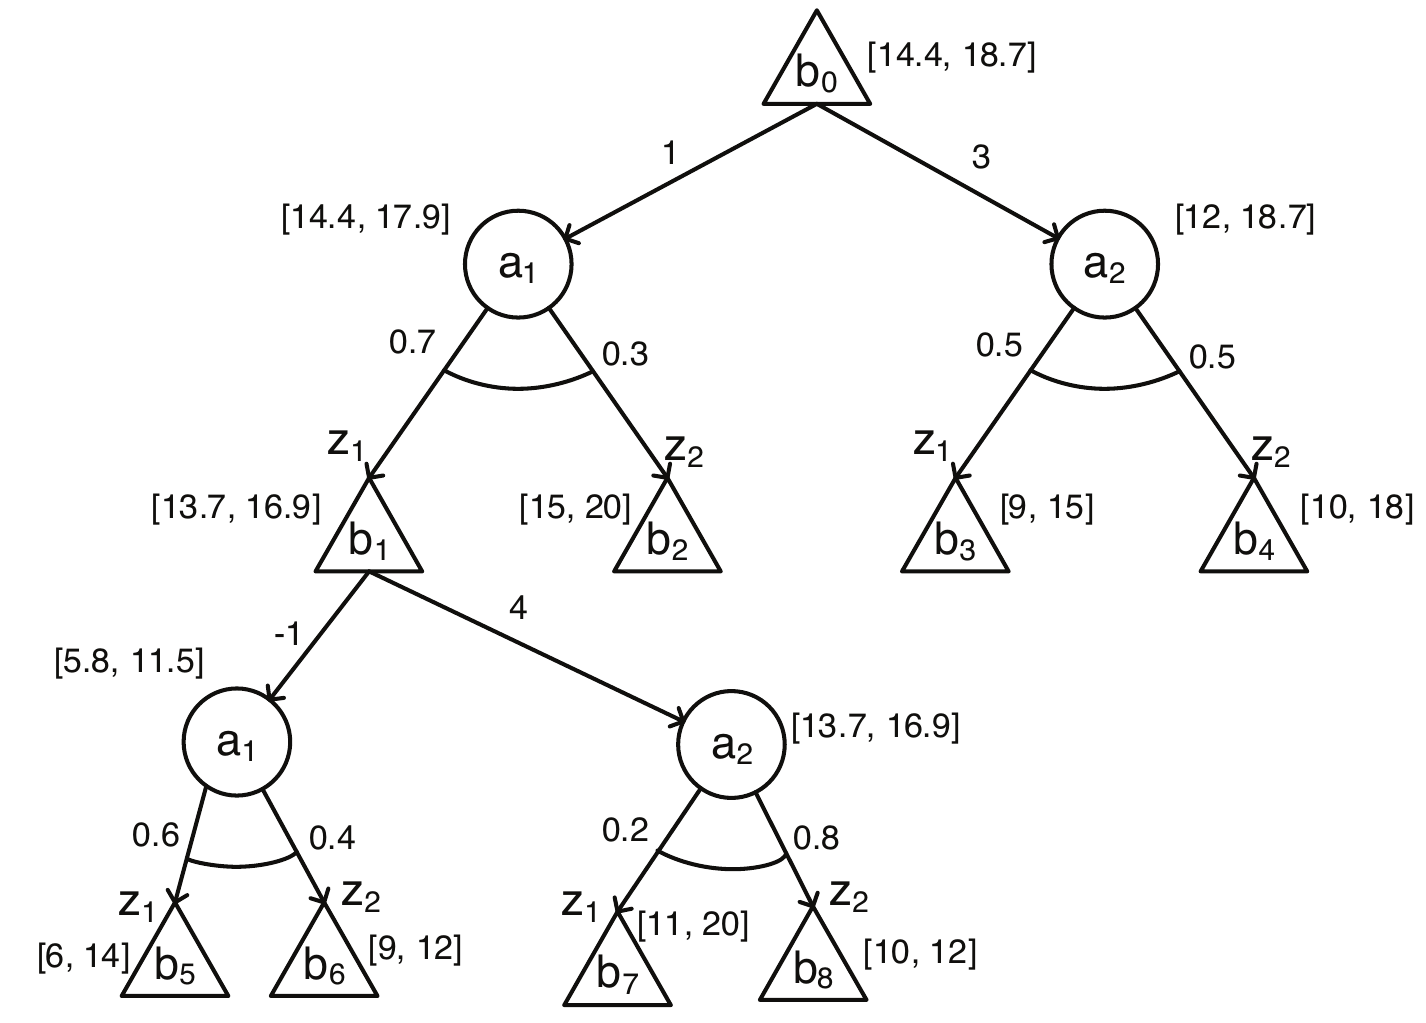
\includegraphics[scale=0.2]{and_or_tree}
\end{figure}

\end{frame}

\begin{frame}
\frametitle{Monte Carlo Tree Search (MCTS): Selection}
\begin{figure}
    \centering
    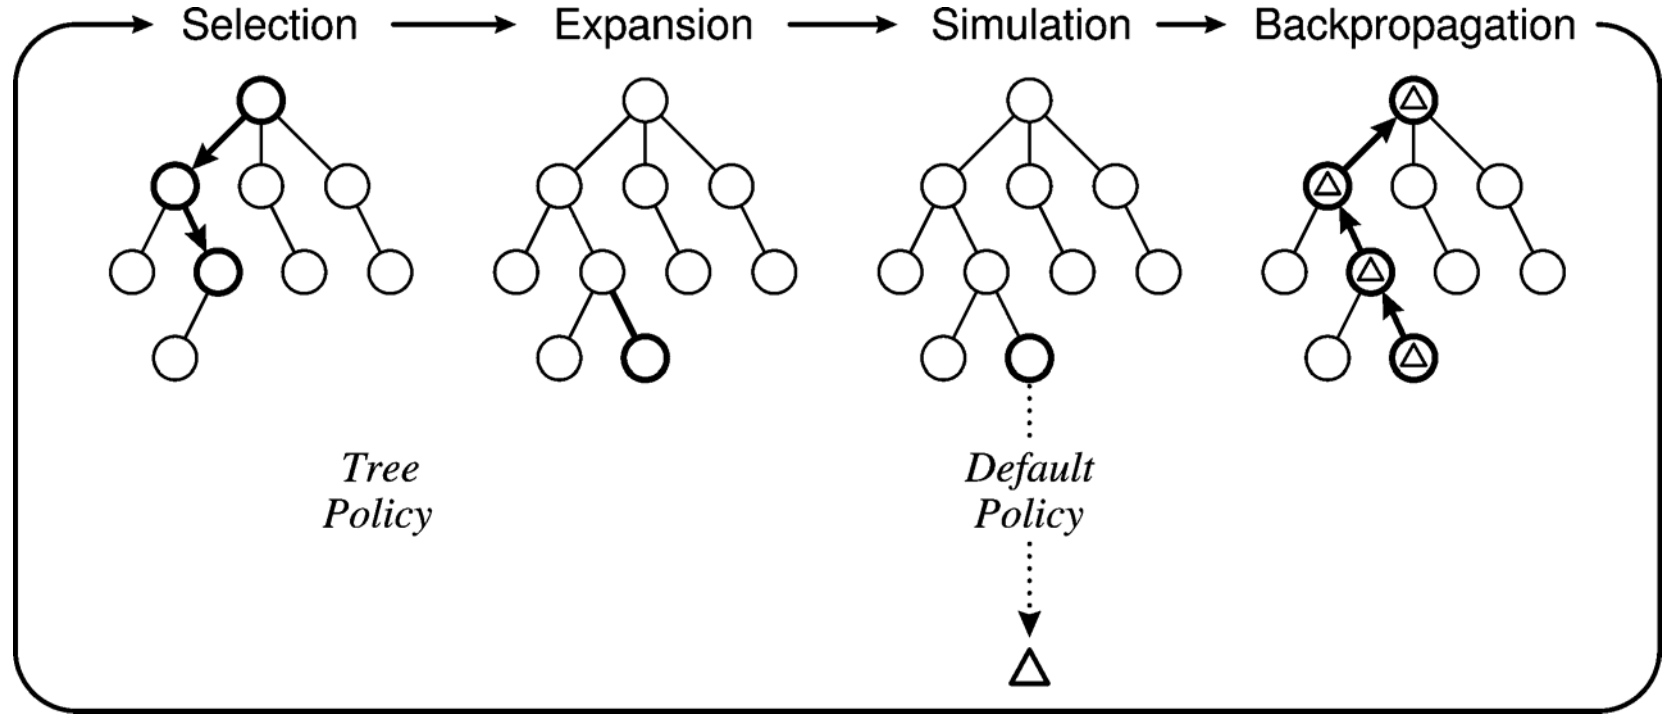
\includegraphics[scale=0.25]{mcts_steps}
\end{figure}

1) Selection:
\small
\begin{itemize}
\item starting at the root node, a child selection policy is recursively applied to descend through the tree until
the most urgent expandable node is reached
\item a node is expandable if it represents a nonterminal state and has unvisited (i.e., unexpanded) children.
\end{itemize}
\end{frame}

\begin{frame}
\frametitle{Monte Carlo Tree Search (MCTS): Expansion}
\begin{figure}
    \centering
    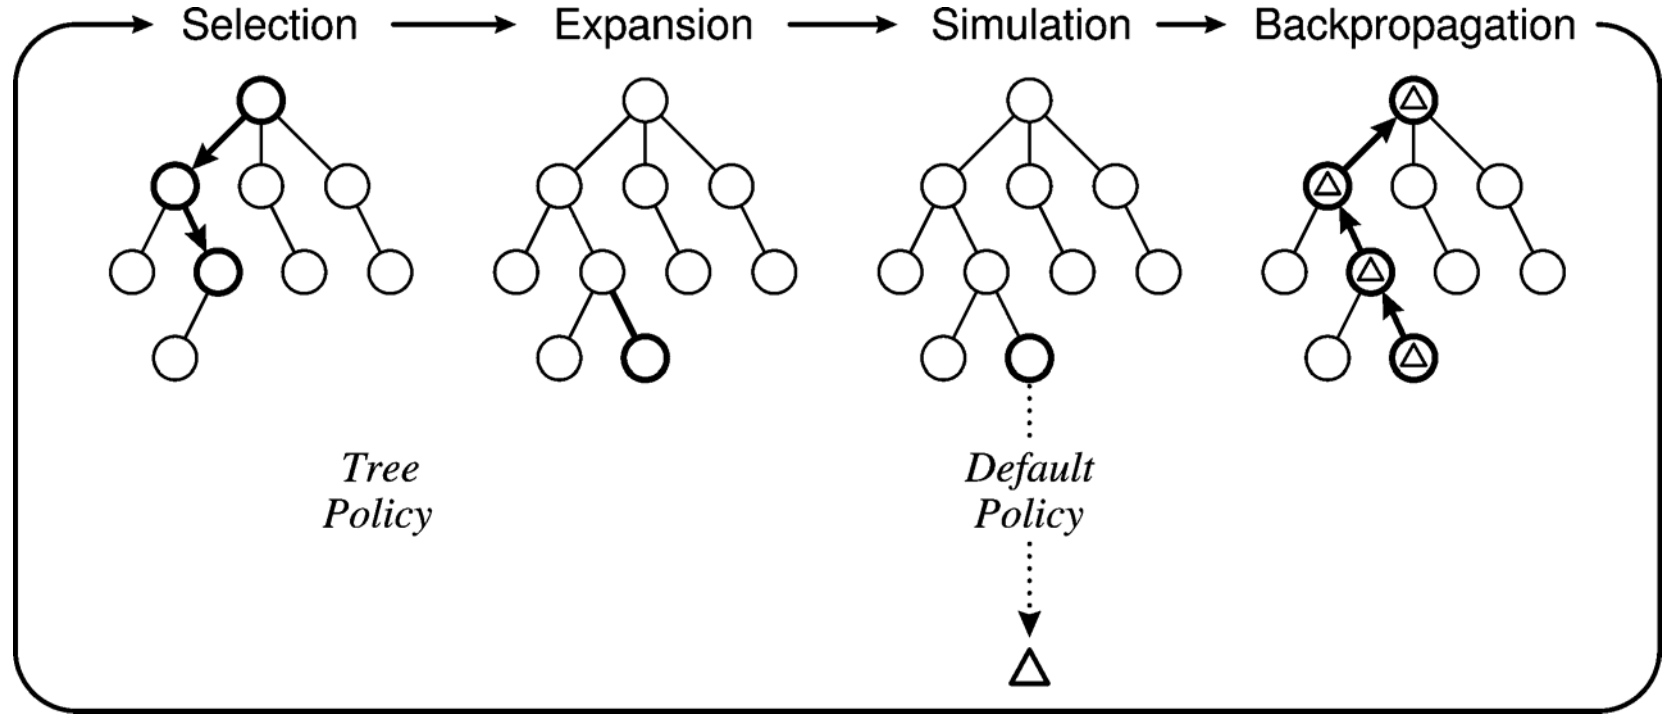
\includegraphics[scale=0.25]{mcts_steps}
\end{figure}

2) Expansion:
\small
\begin{itemize}
\item one (or more) child nodes are added to expand the tree, according to the available actions.
\end{itemize}
\end{frame}

\begin{frame}
\frametitle{Monte Carlo Tree Search (MCTS): Simulation}
\begin{figure}
    \centering
    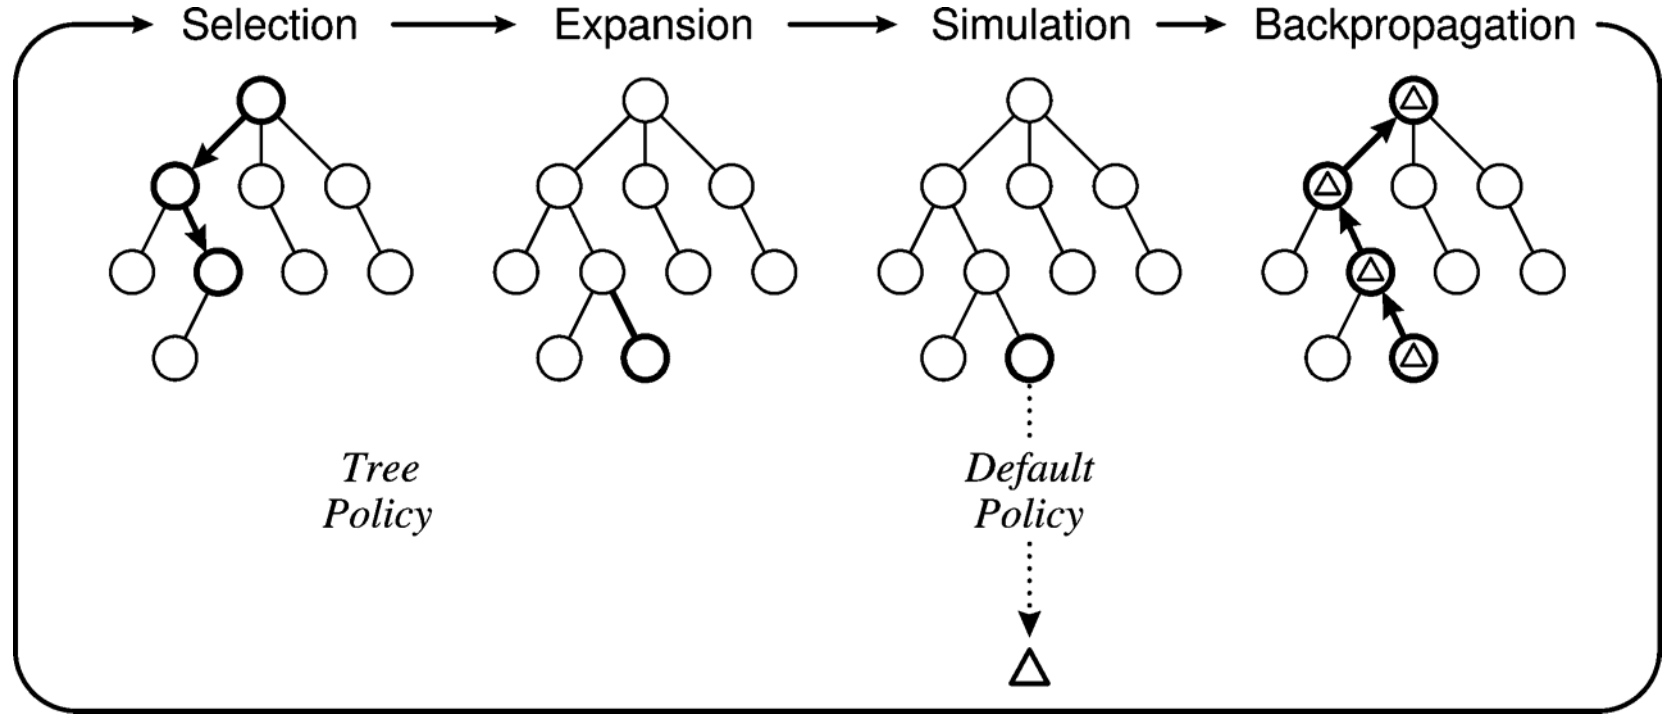
\includegraphics[scale=0.25]{mcts_steps}
\end{figure}

3) Simulation:
\small
\begin{itemize}
\item A simulation is run from the new node(s) according to the default policy to produce an outcome.
\end{itemize}
\end{frame}

\begin{frame}
\frametitle{Monte Carlo Tree Search (MCTS): Backpropagation}
\begin{figure}
    \centering
    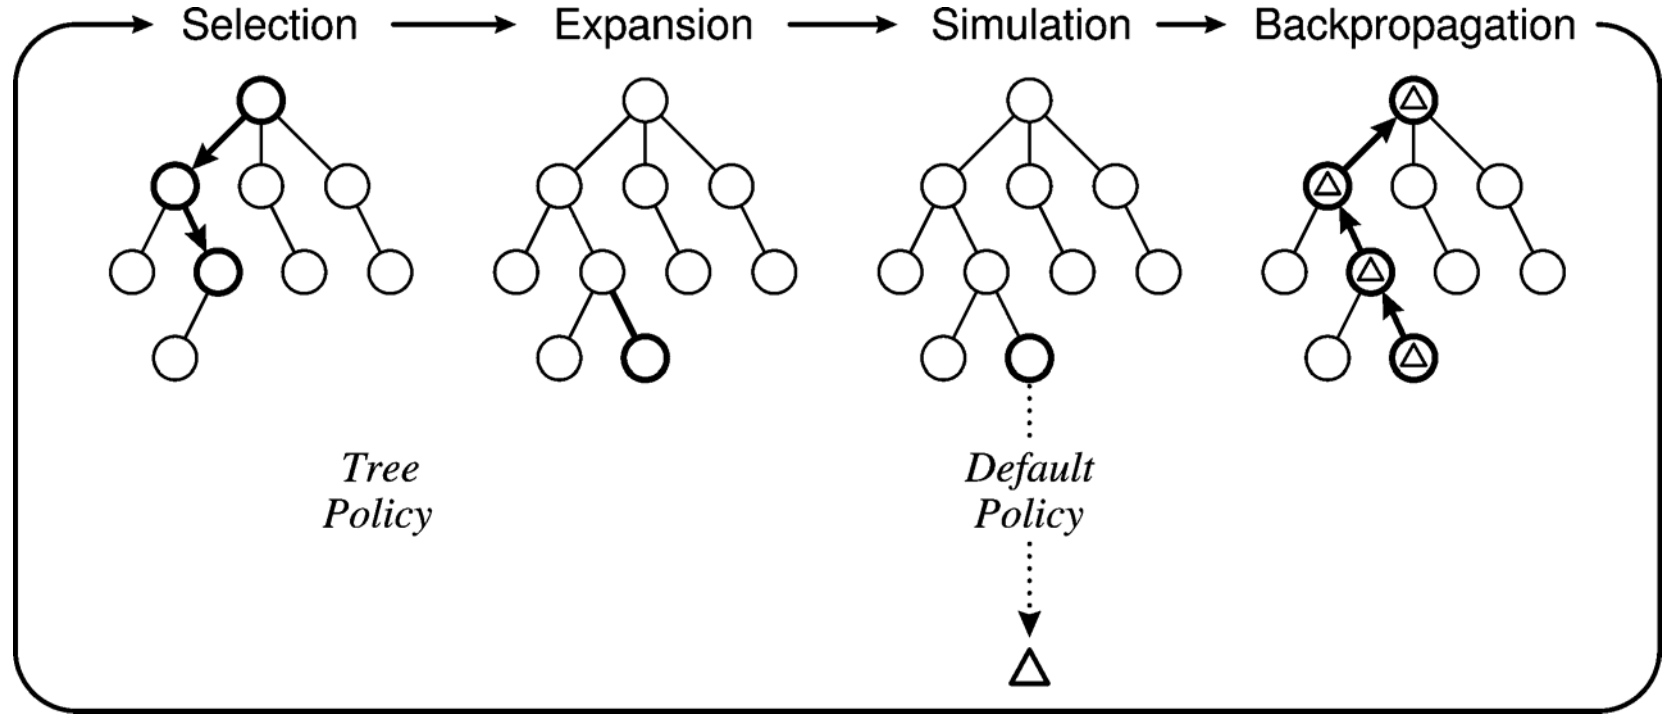
\includegraphics[scale=0.25]{mcts_steps}
\end{figure}

4) Backpropagation:
\small
\begin{itemize}
\item The simulation result is ``backed up'' (i.e., backpropagated) through the selected nodes to
update their statistics.
\end{itemize}
\end{frame}

\begin{frame}
\frametitle{Monte Carlo Tree Search (MCTS): UCT as tree policy}
UCT (UCB1 for Tree): \\
every time a node (action) is to be selected within the existing tree, \\
the choice may be modeled as an independent multiarmed bandit problem \\
\vspace{5mm}
\pause

A child node $j$ is selected to maximize:
\begin{equation*}
UCT = \bar{X}_j + 2 C_p \sqrt{\frac{2~ln~n}{n_j}}
\end{equation*}
\pause

\begin{itemize}
\item $\bar{X}_j$: the average reward from child node $j$ \pause
\item $n$: the number of times the current (parent) node has been visited, \pause
\item $n_j$: the number of times child node $j$ has been visited, \pause
\item $C_p > 0$: a constant.
\end{itemize}

\end{frame}
\section{Partially Observable Monte Carlo Planning (POMCP)}
\frame{\tableofcontents[currentsection, hideothersubsections]}

\begin{frame}
\frametitle{POMCP: Key ideas}
POMCP extends \textbf{MCTS} to \textbf{partially observable} environments
\pause
\begin{itemize}
    \item sample start states from the belief state \\
    (break the curse of dimensionality) \pause
    \item sample histories using a black box simulator \\
    (break the curse of history) \pause
    \item evaluate each state in a search tree by the \textbf{average outcome} of simulations from that state
\end{itemize}

\end{frame}

\begin{frame}
\frametitle{POMCP: $|S|= 50$, $|A|=2$, $|Z|=2$, {\small no intermediate rewards}}
\begin{columns}
  \column{0.5\textwidth}
    \begin{figure}
        \centering
        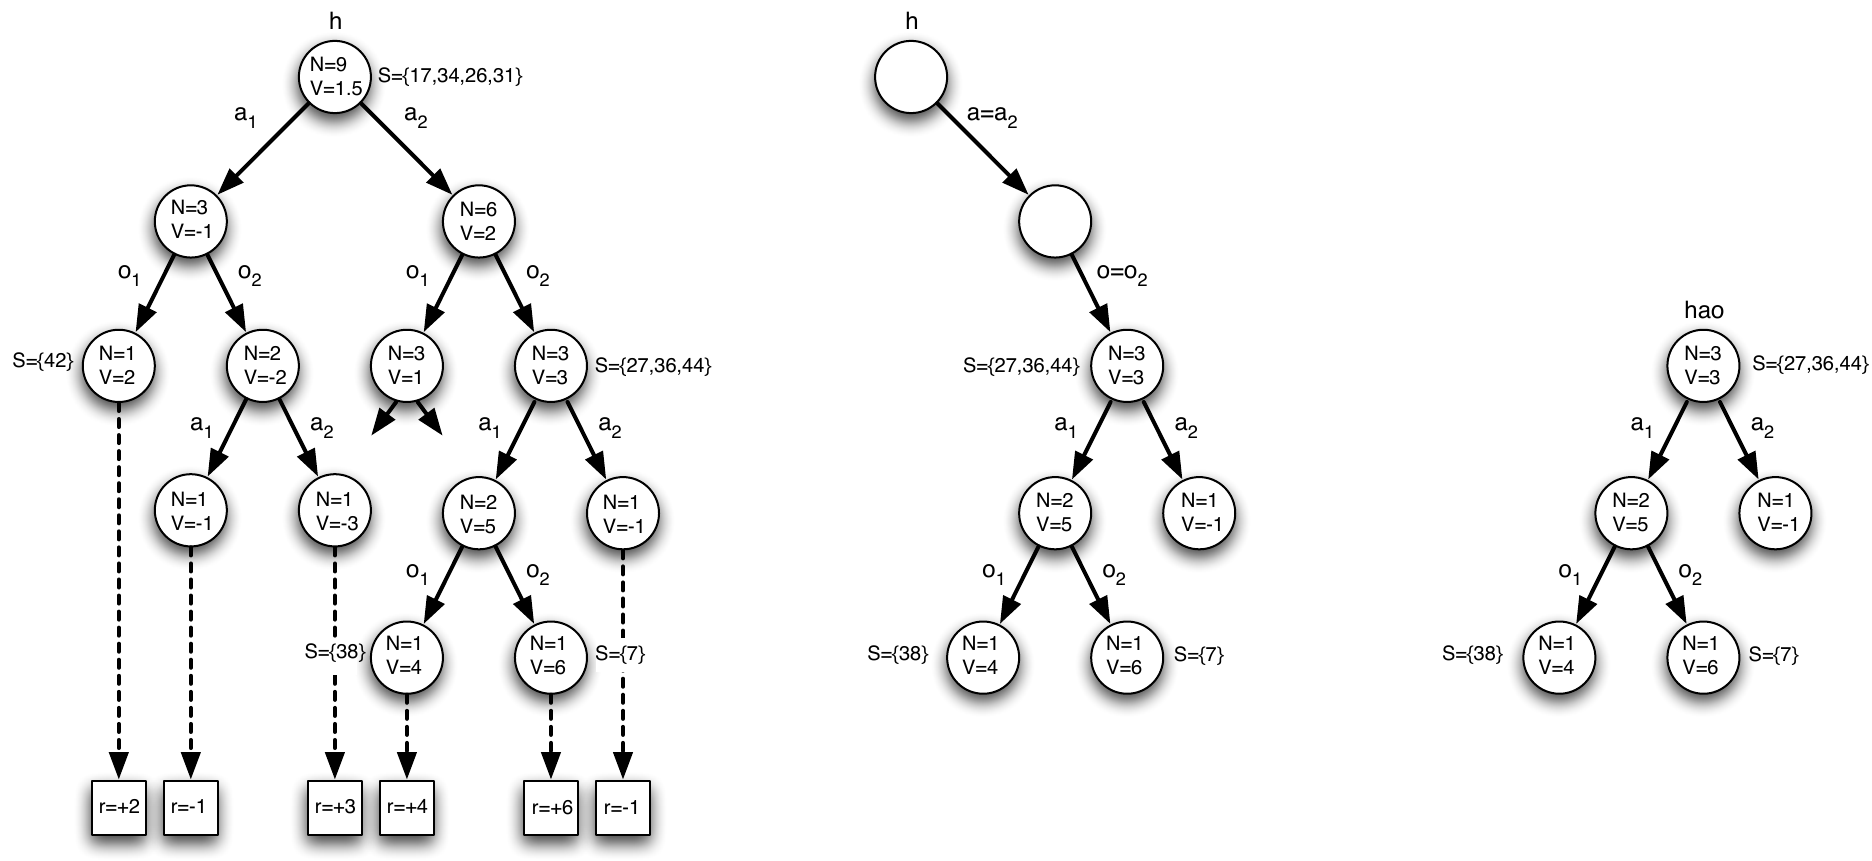
\includegraphics[scale=0.3,trim={0 0 30cm 0},clip]{pomcp_illustration}
    \end{figure}
  \column{0.5\textwidth}
    \begin{itemize}
        \item construct a search tree from multiple simulations, and
        \item evaluate each history by its mean return
    \end{itemize}
\end{columns}
\end{frame}

\begin{frame}
\frametitle{POMCP: $|S|= 50$, $|A|=2$, $|Z|=2$, {\small no intermediate rewards}}
\begin{columns}
  \column{0.5\textwidth}
    \begin{figure}
        \centering
        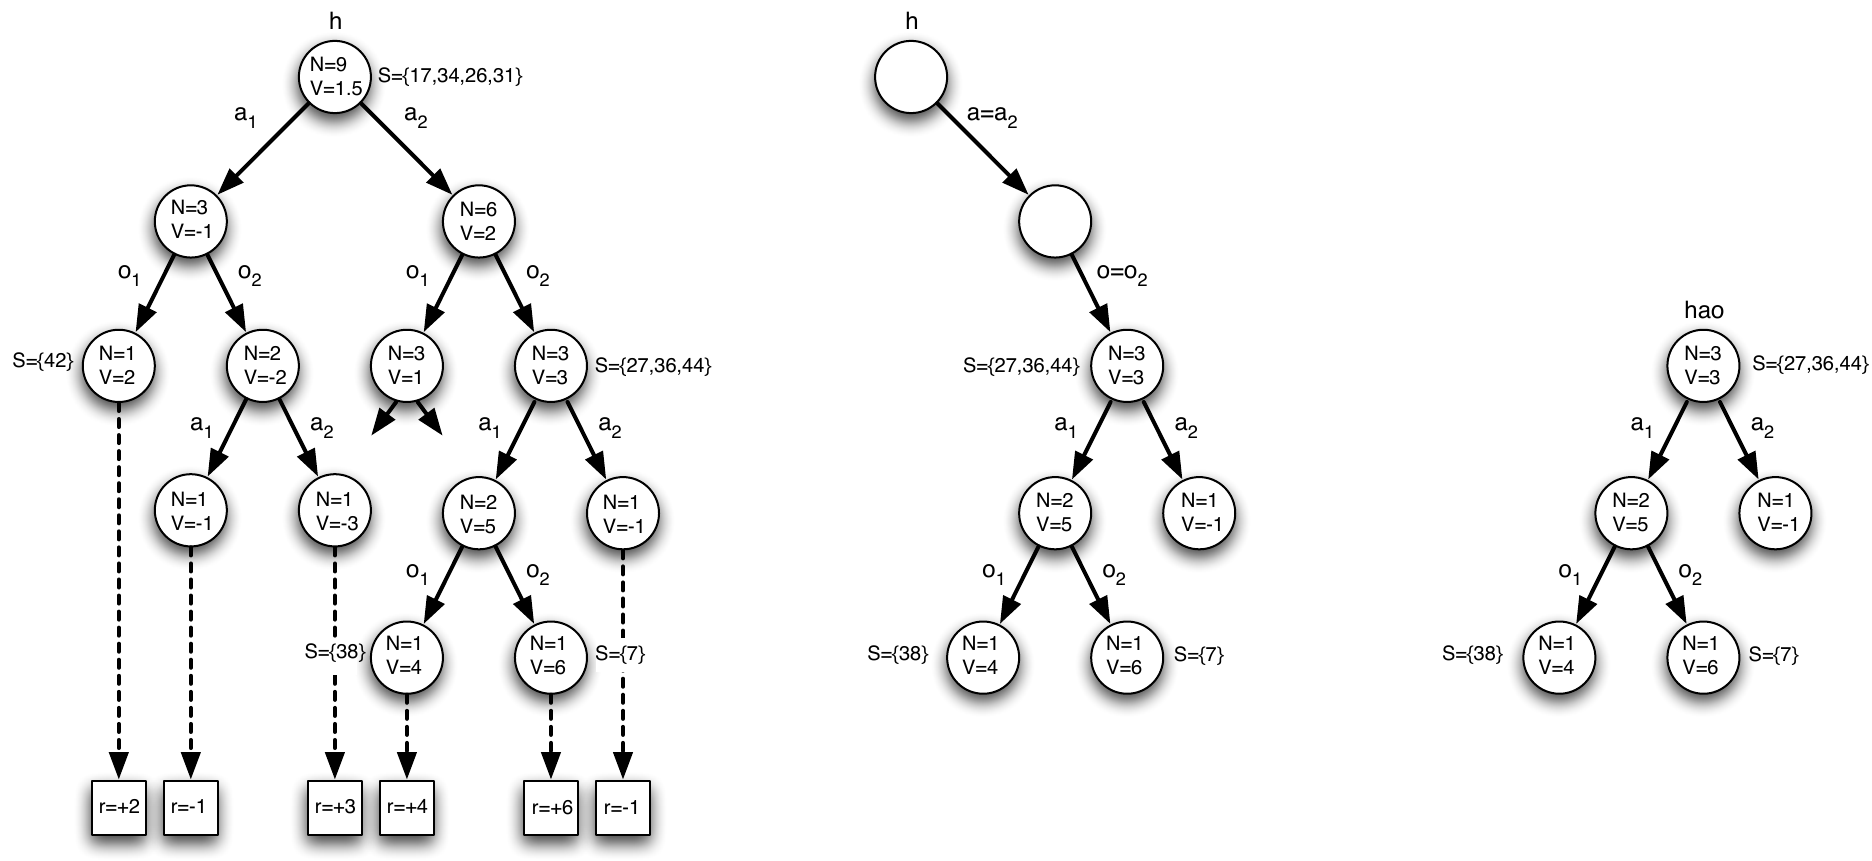
\includegraphics[scale=0.3,trim={20cm 0 15cm 0},clip]{pomcp_illustration}
    \end{figure}
  \column{0.5\textwidth}
    \begin{itemize}
        \item select a real action $a$, and
        \item observe a real observation $o$
    \end{itemize}
\end{columns}
\end{frame}

\begin{frame}
\frametitle{POMCP: $|S|= 50$, $|A|=2$, $|Z|=2$, {\small no intermediate rewards}}
\begin{columns}
  \column{0.5\textwidth}
    \begin{figure}
        \centering
        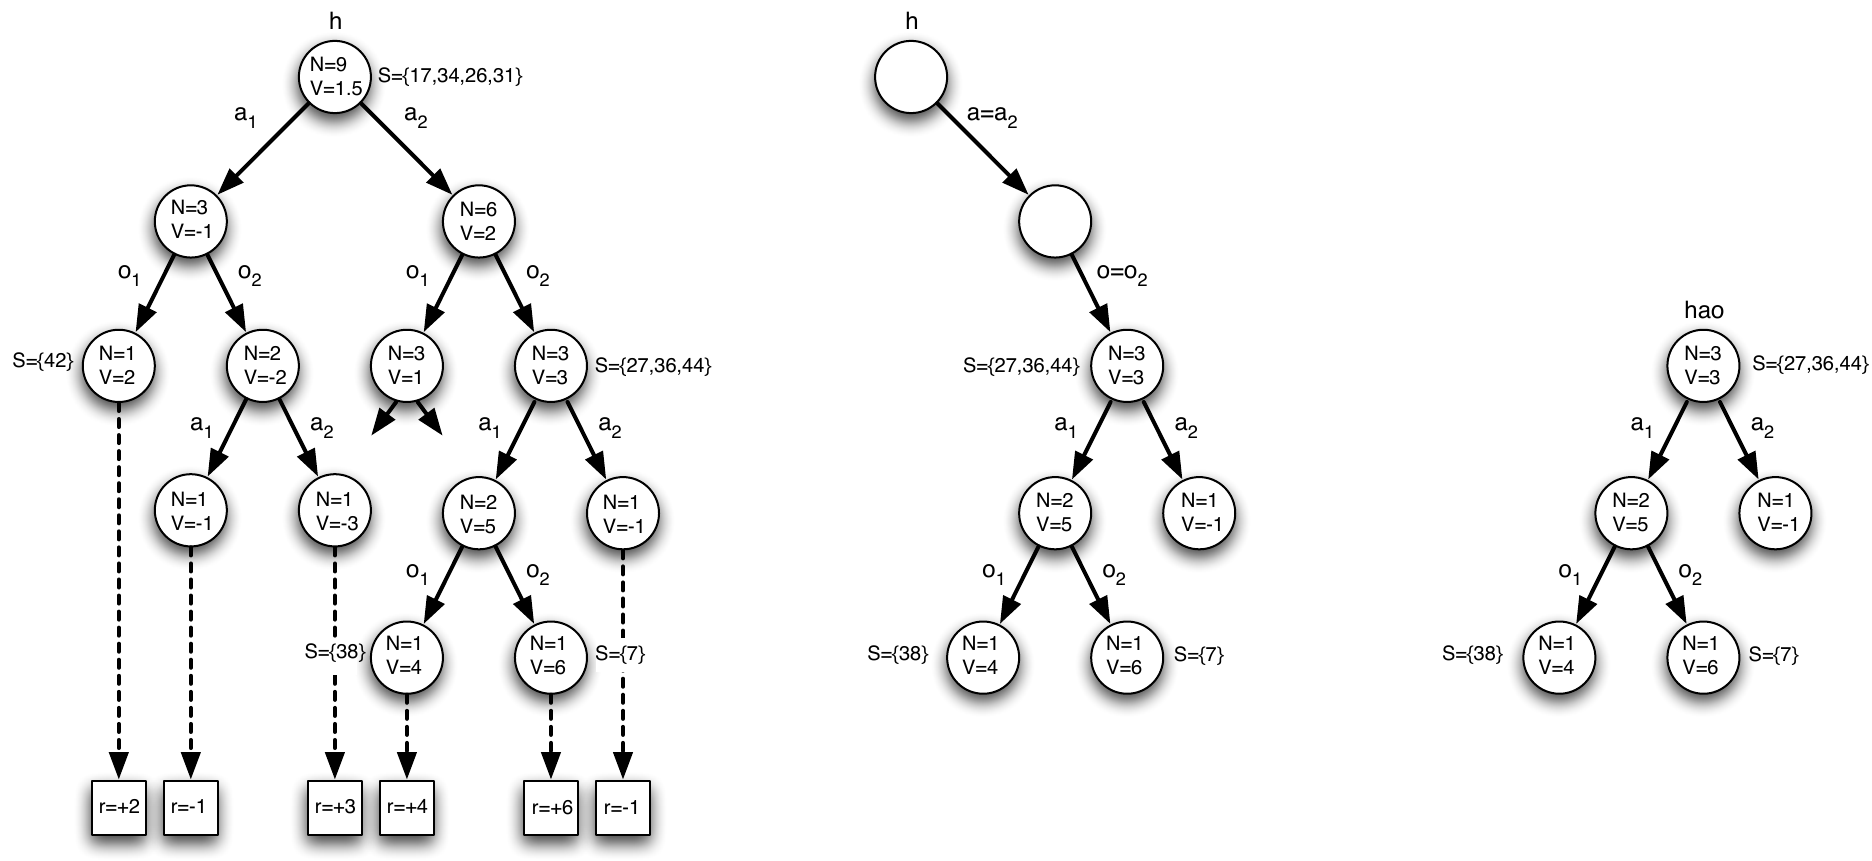
\includegraphics[scale=0.3,trim={35cm 0 0 0},clip]{pomcp_illustration}
    \end{figure}
  \column{0.5\textwidth}
    \begin{itemize}
        \item prune the tree and
        \item begin a new search from the updated history $hao$
    \end{itemize}
\end{columns}
\end{frame}

\begin{frame}
\frametitle{POMCP: algorithm}
\begin{figure}
    \centering
    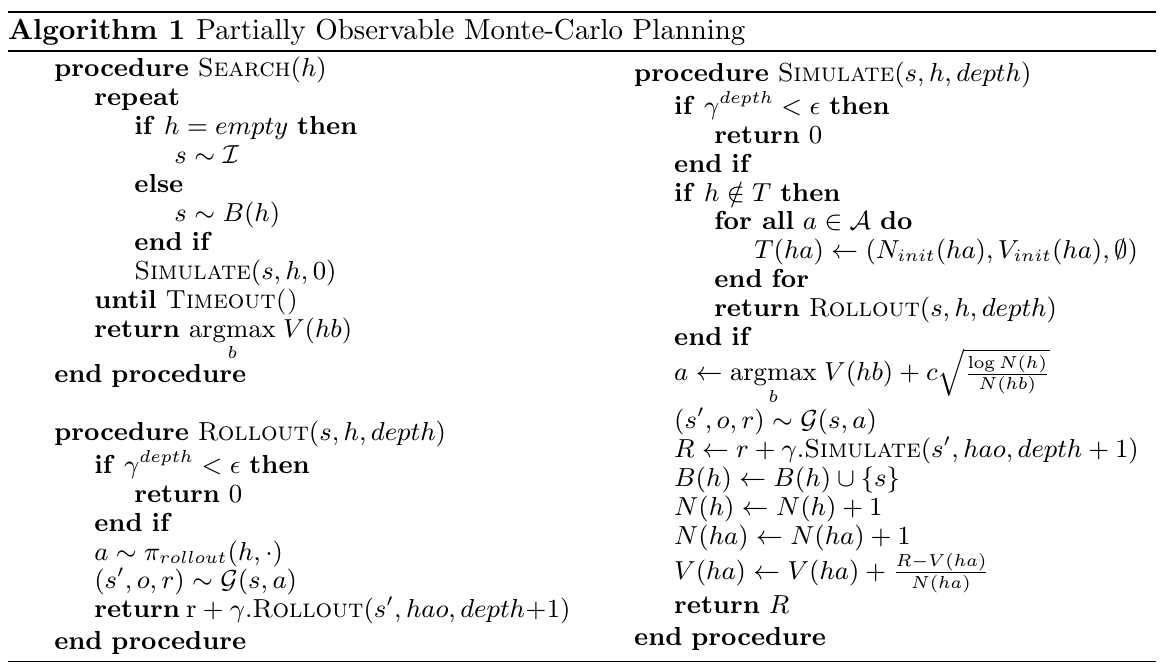
\includegraphics[scale=0.4]{pomcp_algo}
\end{figure}
\end{frame}

\section{Going Further ...}
\frame{\tableofcontents[currentsection, hideothersubsections]}
\section{Conclusions}
\frame{\tableofcontents[currentsection, hideothersubsections]}

\begin{frame}
\frametitle{Conclusions}
?
\end{frame}

\begin{frame}
\Huge{\centerline{Discussion time and thank you.}}
\end{frame}
% \begin{frame} [allowframebreaks]
\frametitle{References}
{\tiny
\bibliographystyle{apacite}
\bibliography{ref}
}
\end{frame}

%%%%%%%%%%%%%%%%%%%%%%%%%%%%%%%%%%%%%%%%%%%%%%%%%%%%%%%%%%%%%%%%%%%%%%%%%%%%%%%

\end{document}
